\section{Multicopter Models}\label{sec:RealizationModels}

\subsection{Actuator models}

\paragraph{Propeller motor.}
The propellers are mounted on a small brushless DC motor (BLDC) which is controlled by dedicated BLDC driver electronics.
This driver implements the electronic commutation and a digital current control with sampling frequency of $64\,\unit{kHz}$.
It gets the desired current $\BLDCCurr$ from the maincontroller with the sampling frequency of $200\,\unit{Hz}$. 
Consequently we assume that all electrical dynamics of the propeller drive are negligible on the timescale of the main controller and the motor torque on the propeller is
\begin{align}
 \BLDCTorque = \BLDCTorqueConstant \BLDCCurr.
\end{align}
\fixme{friction}

\paragraph{Servo motor.}
On the \Tricopter there are servo motors controlling the tilt $\aServo$ of the propellers.
These are standard hobbyist servos witch combine a small motor, a gearbox, a potentiometer and some digital controller which takes the desired servo angle $\aServoR$ as input.
The integrated controller is probably a fast PID controller since it handles constant loads as well as fast transitions quite well.
However, here we assume that the servo torque arises from a simple PD-controller
\begin{align}
 \ServoTorque = \ServoKP (\aServoR - \aServo) - \ServoKD \aServod.
\end{align}
\fixme{blah validation}

\subsection{Propeller aerodynamics}
Here we like to model the propellers, \ie the forces and torques resulting from its rotation.
A general theory of propellers is quite sophisticated, see \eg \cite{Johnson:HelicopterTheory}.
However, for the small, rigid propellers used here (and most common for multicopters of this size) and for the working regime of this text it is sufficient to consider a very simple model:
\begin{align}
 \PropForce = \kappaF \PropVel^2,
\qquad
 \PropTorque = -\kappaT \PropVel^2.
\end{align}
where $\PropVel$ is the angular velocity of the propeller.
The propeller thrust $\PropForce$ is directed along its spinning direction and the propeller drag $\PropTorque$ acts opposing the spinning direction.
The model parameters $\kappaF$ and $\kappaT$ arise from the propeller geometry but will be identified in dedicated experiments.
This model is quite common within the corresponding literature, it is also used in \eg \cite{Mahony:Quadrotor2002}, \cite{MellingerIJRR12} or \cite{Fritsch:Diss}.

In \cite{Bristeau:Propeller} and \cite{Martin:AccelerometerFeedback} a more sophisticated aerodynamic model for a quadcopter of about the same size as the one used here is proposed.
It mainly adds dissipative forces that are bilinear in the propeller velocities $\PropVel$ and the rigid body velocities $\v$ and $\w$.
For this it introduces 8 additional constant model parameters.
Even though their model has a nice physical derivation it does not fit to the experimental observations done for this work.

\fixme{It does, however, give a physical motivation for linear drag on the multicopter body.}

\subsection{Dissipative forces}
We assume a linear damping model for the overall multicopter
\begin{align}
 \begin{bmatrix} \bodyForceSym_D \\ \bodyTorqueSym_D \end{bmatrix}
 &= 
 \begin{bmatrix} D_v & D_v \wedOp(\bodyCOD{}{})^\top \\ \wedOp(\bodyCOD{}{}) D_v & \bodyMOD{}{} \end{bmatrix}
 \begin{bmatrix} \v \\ \w \end{bmatrix}
\end{align}
where $D_v = \diag(\dvx, \dvx, \dvz)$, $\bodyCOD{}{}{} = [0,0,\lz]^\top$, $\bodyMOD{}{}{} = \diag(\sigx, \sigx, \sigz)$.



\subsection{Rigid body model}
A rigid body model for a generic multicopter with tiltable propellers has been extensively discussed in \autoref{sec:RBSRigidBodySys}.
The rigid body model for the \Quadcopter and \Tricopter arises by setting special parameter values.

\paragraph*{Coordinates and Kinematics.}
We choose the configuration coordinates 
\begin{align}
 \sysCoord = \big[ \r^\top, \vectorize(\R)^\top, \PropTilt^\top, \PropAngle^\top \big]^\top \in \RealNum^{12+2\numProp}
\end{align}
where $\r \in \RealNum^3$ is the position of the center body, $\R \in \SpecialOrthogonalGroup(3)$ its orientation matrix, $\PropTilt = [\PropTilt[1], \ldots, \PropTilt[\numProp]]^\top \in \RealNum^{\numProp}$ the arm tilt angles and $\PropAngle = [\PropAngle[1],\ldots,\PropAngle[\numProp]]^\top \in \RealNum^{\numProp}$ the angles of the propellers, see \autoref{fig:TricopterInputs}.
Note that the propellers are asymmetric, \ie designed only for either clockwise or counter-clockwise rotation, and will only rotate in this direction during operation.
The propeller angles $\PropAngle[k]$ are defined, such that $\PropAngled[k] > 0$ during operation.
To recover the spinning directions we use the parameter $\PropDir[k] = 1$ for a positive/counter-clockwise and $\PropDir[k] = -1$ for a negative/clockwise spinning propeller.
\begin{figure}[ht]
 \centering
 \input{graphics/TricopterInputs.pdf_tex}
 \caption{Mechanical model of the \Tricopter}
 \label{fig:TricopterInputs}
\end{figure}

To capture the velocity state of the system we use the velocity coordinates
\begin{align}
 \sysVel = \big[ \v, \omega, \PropTiltd, \PropVel]^\top \in \RealNum^{6+2\numProp},
\end{align}
related to the configuration coordinates by
\begin{align}
 \rd = \R \v, 
\qquad
 \Rd = \R \wedOp(\w),
\qquad
 \PropAngled = \PropVel.
\end{align}

\paragraph{Kinetic equation.}
The algorithm proposed in \autoref{sec:RBSRigidBodySys} does of course handle general mass distributions of the rigid bodies, but the resulting kinetic equations are far too cumbersome to display here explicitly.
Instead we do some assumptions on the body inertia matrices that will lead to a condensed system inertia matrix:
We assume that the combined center of mass of one arms and its propeller lies on the tilt axis.
This already implies that the overall center of mass $\bodyCOM{}{}{} \in \RealNum^{3}$ of the system is constant \wrt the body fixed frame.
This was one goal during the construction process of the Tricopter.
Furthermore, we assume that the combined moment of inertia of one arm and propeller is symmetric about the tilt axis.
This is not the case for the real inertia parameters.
However, it is justified by the fact that the overall inertia $\bodyMOI{}{}{}$ changes only slightly depending on the arm tilts $\PropTilt$ or the propeller angles $\PropAngle$.  
A crucial thing to get the overall dynamics right is to consider the rotor of the servo motor.
The relevant moment of inertia $\bodyMOISym_{\textsf{Sxx}}$ might be very small, but since it is located behind a gearbox with transmission ratio $c_{\mathsf{S}} = 625$ its contribution to the system inertia matrix is significant.
The validity of the model with these assumptions will be discussed later by comparison to experimental data.

With the above assumptions the kinetic equation for the multicopter takes the form
\begin{align}\label{eq:RealizationMulticopterKinetics}
 \sysInertiaMat(\PropTilt) \sysVeld + \gyroForce(\PropTilt, \sysVel) + \sysDissMat \sysVel + \genForceGravity(\R) &= \genForceProp(\PropTilt, \PropVel) + \genForceInput(\BLDCTorque, \ServoTorque) + \genForceBias
\end{align}
where
\begin{subequations}\label{eq:RealizationMulticopterForces}
\begin{align}
 \sysInertiaMat(\PropTilt) &=
 \begin{bmatrix}[1.1]
  \m \idMat[3] & \m \wedOp(\bodyCOM{}{})^\top & 0 & 0 \\
  \m \wedOp(\bodyCOM{}{}) & \bodyMOI{}{}{} & \JAC H_1 & \JP H_3(\PropTilt) \diag(\PropDir) \\
  0 & \JAC H_1^\top & \ArmInertia \idMat[\numProp] & 0 \\
  0 & \JP \diag(\PropDir) H_3^\top(\PropTilt) & 0 & \PropInertia \idMat[\numProp]
 \end{bmatrix},
\\
 \gyroForce(\PropTilt, \sysVel) &= 
 \begin{bmatrix}[1.1]
  \wedOp(\w) \genMomentumSym_{\v} \\
  \wedOp(\v) \genMomentumSym_{\v} + \wedOp(\w) \genMomentumSym_{\w} + \JP H_4(\PropTilt) \diag(\PropTiltd) \diag(\PropDir) \PropVel \\
  -\JP \diag( \diag(\PropDir) H_4^\top(\PropTilt) \w) \PropVel \\
   \JP \diag( \diag(\PropDir) H_4^\top(\PropTilt) \w) \PropTiltd \\
 \end{bmatrix},
\\
 \sysDissMat &= \begin{bmatrix} D_v & D_v \!\wedOp(\bodyCOD{}{})^\top\! & 0 & 0 \\ \wedOp(\bodyCOD{}{}) D_v & \bodyMOD{}{}{} & 0 & 0 \\ 0 & 0 & 0 & 0 \\ 0 & 0 & 0 & 0 \end{bmatrix}\!,
\quad
 \genForceGravity(\R) = \begin{bmatrix}[1.1] \m \idMat[3] \\ \m \wedOp(\bodyCOM{}{}) \\ 0 \\ 0 \end{bmatrix} \RT (-\gravityAcc),
\\
 \genForceProp(\PropTilt, \PropVel) &= \begin{bmatrix} \kappaF H_3(\PropTilt) \\ \kappaF \big( \ArmRadius H_4(\PropTilt) + \ArmHeight H_2(\PropTilt) \big) - \kappaT H_3(\PropTilt) \diag(\PropDir) \\ 0 \\ -\kappaT \idMat[\numProp] \end{bmatrix} \diag(\PropVel) \PropVel,
\\
 \genForceInput(\BLDCTorque, \ServoTorque) &= \begin{bmatrix} 0 \\ 0 \\ \ServoTorque \\ \BLDCTorque \end{bmatrix}
\qquad
 \genForceBias = \begin{bmatrix} \FB \\ \tauB \\ 0 \\ \BLDCFriction \end{bmatrix}
\end{align}
with the (just for readability) substituted momenta
\begin{align}
 \genMomentumSym_{\v} &= m (\v - \wedOp(\bodyCOM{}{}) \w), 
\\
 \genMomentumSym_{\w} &= m \wedOp(\bodyCOM{}{}) \v + \bodyMOI{}{}{} \w + \JAC H_1 \PropTiltd  + \JP H_3(\PropTilt) \diag(\PropDir) \PropVel.
\end{align}
and the sub-matrices
\begin{align}
 H_1 &= \begin{bmatrix}
  \cArmAngle[1] & \cdots & \cArmAngle[\numProp] \\
  \sArmAngle[1] & \cdots & \sArmAngle[\numProp] \\
  0 & \cdots & 0
 \end{bmatrix}\!,&
 H_2(\PropTilt) &= \begin{bmatrix}
  \cArmAngle[1] \sPropTilt[1] & \cdots & \cArmAngle[\numProp] \sPropTilt[\numProp] \\
  \sArmAngle[1] \sPropTilt[1] & \cdots & \sArmAngle[\numProp] \sPropTilt[\numProp] \\
  0 & \cdots & 0
 \end{bmatrix}\!,
\\
 H_3(\PropTilt) &= \begin{bmatrix}
   \sArmAngle[1] \sPropTilt[1] & \cdots &  \sArmAngle[\numProp] \sPropTilt[\numProp] \\
  -\cArmAngle[1] \sPropTilt[1] & \cdots & -\cArmAngle[\numProp] \sPropTilt[\numProp] \\
   \cPropTilt[1]               & \cdots &  \cPropTilt[\numProp]                     
 \end{bmatrix}\!,&
 H_4(\PropTilt) &= \begin{bmatrix}
  \sArmAngle[1] \cPropTilt[1] & \cdots & \sArmAngle[\numProp] \cPropTilt[\numProp] \\
  -\cArmAngle[1] \cPropTilt[1] & & -\cArmAngle[\numProp] \cPropTilt[\numProp] \\
  -\sPropTilt[1] & \cdots & -\sPropTilt[\numProp]
 \end{bmatrix}
% \quad \tdiff{t} \big( H_3(\PropTilt) \big) = H_3'(\PropTilt) \diag(\PropTiltd)
\end{align}
\end{subequations}

\paragraph{Tricopter.}
To get the rigid body model equations for the Tricopter (displayed in \autoref{fig:TricopterInputs}) we can plug the following parameters into \eqref{eq:RealizationMulticopterForces}
\begin{align}
 \numProp = 3,
\qquad
%  \ArmAngle[1] = \tfrac{\pi}{3}, \
%  \ArmAngle[2] = \pi, \
%  \ArmAngle[3] = -\tfrac{\pi}{3},
 \ArmAngle = \tfrac{\pi}{3} [1, 3, 5]^\top,
\qquad
%  \PropDir[1] = -1, \
%  \PropDir[2] = \PropDir[3] = 1.
 \PropDir = [-1, +1, +1]^\top.
\end{align}
However, the model equations do not simplify too much and are not displayed explicitly here.

\paragraph{Quadcopter.}
For the Quadcopter model we have the parameters (see \autoref{fig:QuadcopterInputs})
\begin{align}
 \numProp = 4,
\qquad
%  \ArmAngle[1] = 0, \
%  \ArmAngle[2] = \tfrac{\pi}{2}, \
%  \ArmAngle[3] = \pi, \
%  \ArmAngle[4] = -\tfrac{\pi}{2},
 \ArmAngle = \tfrac{\pi}{2} [0, 1, 2, 3]^\top,
\qquad
%  \PropDir[1] = \PropDir[3] = 1, \
%  \PropDir[2] = \PropDir[4] = -1,
 \PropDir = [+1, -1, +1, -1]^\top,
\qquad
% \PropTilt[1] = \PropTilt[2] = \PropTilt[3] = \PropTilt[4] = 0.
 \PropTilt = [0, 0, 0, 0]^\top.
\end{align}
Here the model equations simplify significantly.
Since the propellers do not tilt $\PropTilt = 0$, the corresponding equations can be regarded as definition of reaction torques $\ServoTorque$ and dropped from the model equations.
Overall the model for the Quadcopter is
\begin{subequations}
\begin{align}
 \sysInertiaMat &=
 \begin{bmatrix}
  \m \idMat[3] & -\m \wedOp(\bodyCOM{}{}) & 0 \\
  \m \wedOp(\bodyCOM{}{}) & \bodyMOI{}{}{} & \JP H_3 \diag(\PropDir)\\
  0 & \PropInertia \diag(\PropDir) H_3^\top & \PropInertia \idMat[4] \\
 \end{bmatrix},
\\
 \gyroForce(\sysVel) &= 
 \begin{bmatrix} \wedOp(\w) & 0 & 0 \\ \wedOp(\v) & \wedOp(\w) & 0 \\ 0 & 0 & 0 \end{bmatrix}
 \sysInertiaMat \sysVel,
\qquad
 \genForceGravity(\R) = \begin{bmatrix} \m \idMat[3] \\ \m \wedOp(\bodyCOM{}{}) \\ 0 \end{bmatrix} \RT (-\gravityAcc),
\\
 \genForceProp(\PropVel) &= \begin{bmatrix} \kappaF H_3 \\ \kappaF \ArmRadius H_4 - \kappaT H_3 \diag(\PropDir)  \\ -\kappaT \idMat[4]  \end{bmatrix} \diag(\PropVel) \PropVel,
\qquad
 \genForceInput(\BLDCTorque) = \begin{bmatrix} 0 \\ 0 \\ \BLDCTorque \end{bmatrix}
\end{align}
with the sub-matrices
\begin{align}
 H_3 &= \begin{bmatrix}
  0 & 0 & 0 & 0 \\
  0 & 0 & 0 & 0 \\
  1 & 1 & 1 & 1
 \end{bmatrix}\!,&
 H_4 &= \begin{bmatrix}
  0 & 1 & 0 & -1 \\
  -1 & 0 & 1 & 0 \\
  0 & 0 & 0 & 0
 \end{bmatrix}\!.
\end{align}
\end{subequations}
Note that the system inertia matrix $\sysInertiaMat$ is constant, but there is still an inertial coupling between the propeller velocities $\PropVel$ and $\wz$.
The same model up to different dissipative forces has been derived in \cite{Martin:AccelerometerFeedback}.
In \cite{Mahony:Quadrotor2002} a quadcopter model is proposed which is similar ...

\begin{figure}[ht]
 \centering
 \input{graphics/QuadcopterInputs.pdf_tex}
 \caption{Propeller forces on the Quadcopter}
 \label{fig:QuadcopterInputs}
\end{figure}


\subsection{Parameter identification}
The preceding mathematical model for the multicopters contains various constant parameters of which only the total mass $\m$ and the arm radius $\ArmRadius$ can be measured directly.
Some crucial parameters are identified in dedicated experimental setups which will be discussed in the following.
The remaining parameters are estimated by the method of least squares ...

%As mentioned before the overall rigid body system has a constant total mass $\m \in \RealNum$, combined center of mass $\bodyCOM{}{}{} \in \RealNum^3$ and combined moment of inertia $\bodyMOI{}{}{}=\bodyMOI{}{}{}^\top \in\RealNum^{3\times3}$.

\paragraph*{Propeller and servo drive.}
For the identification of the propeller drive and its tilting mechanism we use a dedicated test bench, see \autoref{fig:PropellerTestBench}.
It is essentially one mounted Tricopter arm with additional high resolution sensors for the tilt $\PropTilt$ and propeller velocity $\PropVel$.

\begin{figure}
 \centering
 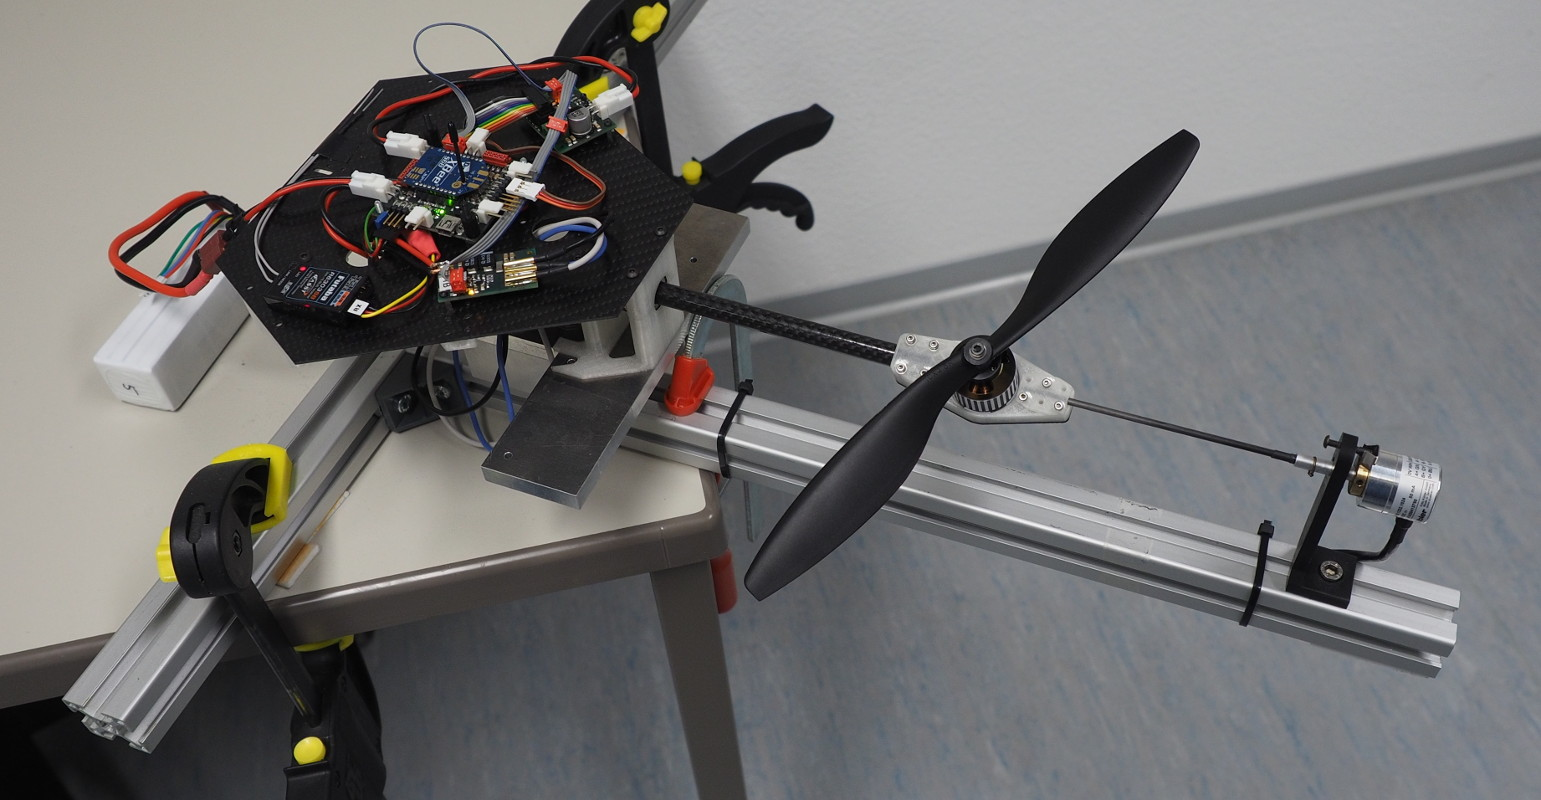
\includegraphics[width=.6\linewidth]{PropellerTestBench.jpg}
 \caption{Test bench for the propeller and tilting mechanism}
 \label{fig:PropellerTestBench}
\end{figure}
 
The equations of motion for the test bench are
\begin{align}
 \PropVeld + \underbrace{\tfrac{\kappaT}{\JP}}_{\PropParam[1]} \PropVel^2 &= \underbrace{\tfrac{\BLDCTorqueConstant}{\JP}}_{\PropParam[2]} \BLDCCurr + \underbrace{\tfrac{\BLDCFriction}{\JP}}_{\PropParam[3]}
\\
 \aServodd + \underbrace{\tfrac{\ServoKD}{\JA}}_{\ServoParam[1]} \aServod + \underbrace{\tfrac{\ServoKP}{\JA}}_{\ServoParam[0]} \aServo &= \underbrace{\tfrac{\ServoKP}{\JA}}_{\ServoParam[0]} \aServoU
\end{align}
The equations are normalized, yielding the parameters $\PropParam[1]$, $\PropParam[2]$, $\PropParam[3]$ and $\ServoParam[0]$, $\ServoParam[1]$, which will become mode convenient later.
These parameters can be directly estimated by the method of least squares.
The inertia parameters $\JP$ and $\JA$ are calculated from the detailed CAD model of the multicopters.
With them one could recover the original parameters $\kappaT$, $\ServoKP$, etc.. 
The identified parameter values are summarized in \autoref{tab:ParamTriQuad}.

The accuracy of the proposed model and its identified parameters can be seen from the results in \autoref{fig:ServoSimRes} and \autoref{fig:PropCtrlRes} in \autoref{sec:RealizationForceVectorControl}.
An online estimation of the bias parameter $\PropParam[3]$ by means of an observer will be discussed there as well.

\paragraph*{Propeller thrust.}
For identification of the thrust constant $\kappaF$, a propeller drive was mounted horizontally on a $1\,\unit{m}$ tall pole.
The pole in turn stands on a digital scale and the ``weight'' was recorded at different propeller speeds $\PropVel$.
From this ``weight'' we can compute the corresponding propeller thrust $\PropForce$.
The measurements are displayed in \autoref{fig:PropVel2Thrust} together with the model $\PropForce = \kappaF \PropVel^2$ with the identified parameter value $\kappaF = 1.44 \cdot 10^{-5}\,\unit{N}\,\unit{s}^2$.

\begin{figure}
 \centering
 \footnotesize%
 \appendtographicspath{{graphics/PropVel2Thrust/}}%
 \begingroup%
\setlength{\unitlength}{1cm}%
\begin{picture}(12.000000,7.000000)%
\put(0,0){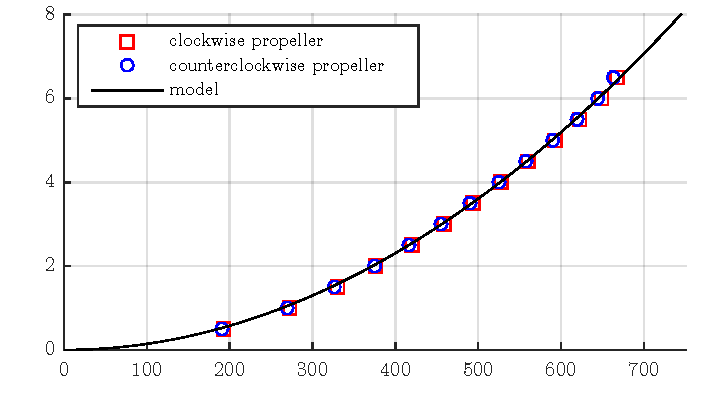
\includegraphics{PropVel2Thrust.pdf}}%
\put(6.327132, 0.157528){\makebox(0,0)[b]{\smash{$\PropVel$ in $\sfrac{\unit{RAD}}{\unit{s}}$}}}%
\put(0.522160, 3.911988){\rotatebox{90}{\makebox(0,0)[t]{\smash{$\PropForce$ in $\unit{N}$}}}}%
\end{picture}%
\endgroup%%
 \caption{Measured propeller thrust compared to proposed model}
 \label{fig:PropVel2Thrust}
\end{figure}

\paragraph*{Rigid body inertia.}
For identification of the inertia parameters $\Jxx$, $\Jyy$ and $\Jzz$ for Tri- and Quadcopter a dedicated experiment was conducted.
The body was suspended by two strings as shown on the left side of \autoref{fig:QuadPendulumIdent}.
The basic idea is that a rotation of the body about the vertical axis results in a upward movement of the body which is countered by gravity.

\begin{figure}[ht]
 \centering
 \input{graphics/QuadPendulumIdent.pdf_tex}
 \hfill
 \footnotesize%
 \appendtographicspath{{graphics/PendulumIdentRes/}}%
 \begingroup%
\setlength{\unitlength}{1cm}%
\begin{picture}(9.000000,6.300000)%
\put(0,0){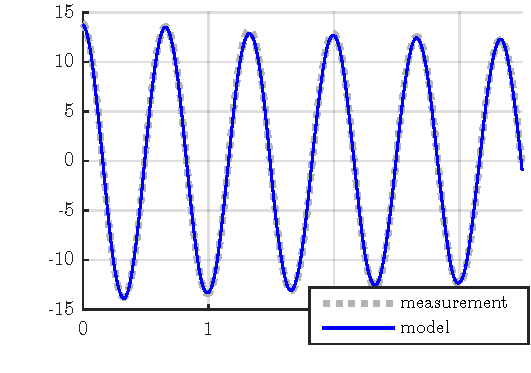
\includegraphics{PendulumIdentRes.pdf}}%
\put(5.099467, 0.138788){\makebox(0,0)[b]{\smash{$t$ in $\unit{s}$}}}%
\put(0.535099, 3.562518){\rotatebox{90}{\makebox(0,0)[t]{\smash{$\ddot{\alpha}$ in $\sfrac{\unit{RAD}}{\unit{s}^2}$}}}}%
\end{picture}%
\endgroup%%
 \caption{Experimental setup and identification result for $\Jxx$ of the Quadcopter}
 \label{fig:QuadPendulumIdent}
\end{figure}

The equation of motion for the vertical rotation with angle $\alpha$ in this setup is
\begin{align}\label{eq:PendulumIdent}
 \bodyMOI{}{}{} \ddot{\alpha} + \m \gravityAccConst \frac{d^2 \sin\alpha}{4\sqrt{h^2 - \tfrac{d^2}{2}(1-\cos\alpha)}} = 0.
\end{align}
Here $\m$ indicated the total mass of the copter, $\gravityAccConst = 9.81\,\sfrac{\unit{m}}{\unit{s}^2}$ is the gravitational acceleration, $d$ and $h$ are the distance and length of the strings.
From the measured trajectory $t\mapsto\alpha$ of the twist angle we can estimate the inertia $\bodyMOI{}{}{}$ about the corresponding axis.
On the right side of \autoref{fig:QuadPendulumIdent}, the acceleration $\ddot{\alpha}$ computed from the model \eqref{eq:PendulumIdent} with the estimated parameters is plotted against the measured acceleration.

This test was conducted for all three axis, \ie for $\Jxx$, $\Jyy$ and $\Jzz$ for Tri- and Quadcopter and the resulting parameters are given in \autoref{tab:ParamTriQuad}.
The identified parameters match the values computed from a detailed CAD model by $\pm 10\%$.

\paragraph*{Parameter identification from flight test.}
The model \eqref{eq:RealizationMulticopterKinetics} still contains several so far unknown parameters:
The coordinates of the center of mass $\bodyCOM{}{}{} = [\sx, \sy, \sz]^\top$, the off-diagonal entries $\Jxy$, $\Jxz$ and $\Jyz$ of the inertia matrix and the inertia parameter $\JAC$.
The translational damping $\dvx$, $\dvz$, the rotational damping $\sigx$, $\sigz$ and the coordinate $\lz$ of the center of damping.

With some auxiliary transformation ($\lzp = \dvx\lz$, $\sigxp = \sigx + \dvz\lz^2$) the first 6 model equations \eqref{eq:RealizationMulticopterKinetics} are linear in the remaining unknown parameters.
So we can identify these by the method of least squares from flight test measurements.
\autoref{tab:ParamTriQuad} summarizes the identified parameter values from this flight test as well as the ones from the previously discussed dedicated experiments.
These are the values that are used for the simulator.

From this experiment we have the first estimate for the overall center of mass $\bodyCOM{}{}{}$ of Tri- and Quadcopter.
The identified value $\sz$ is then used to adjust the body fixed frame in the vertical direction such that $\sz=0\,\unit{m}$.
For the Tricopter this determines also the parameter $\ArmHeight$.
The values for $\sx$ and $\sy$ are small so we stick to the geometric center in the horizontal directions.

The damping parameter values for the Tricopter are greater than the ones for the Quadcopter.
This could be explained by the model from \cite{Martin:AccelerometerFeedback} and the fact that the propellers of the Tricopter nominally spin $40\%$ faster than on the Quadcopter.
Also the identified value for $\lz$ is roughly the distance from the body fixed frame to the propeller plane which fits well to their model.
On the other hand, the identified translational damping $\dvz$ in the vertical direction is greater than the horizontal damping $\dvx$.
This contradicts the model proposed in \cite{Martin:AccelerometerFeedback} which would imply $\dvz = 0$.

\autoref{tab:ParamTriQuad} also shows identified constant bias forces $\FB$ and torques $\tauB$ for this particular experiment.
These mean values probably result from small misalignments of the propellers and servos rather than constant side wind or anything similar.
In the practical application the bias forces will be estimated online by means of an observer, so can vary slowly.
However, the magnitudes of the displayed identified values are less than $3\%$ compared to the maximal available propeller forces $\genForceProp$ in the corresponding directions, so their influence on the overall identification result should be small.



% The scalar inertia parameters
% \begin{align}
%  \JA &= \bodyMOISym_{\mathsf{Axx}} + c_{\mathsf{S}}^2 \bodyMOISym_{\mathsf{Sxx}},&
%  \JAC &= \bodyMOISym_{\mathsf{Axx}} + c_{\mathsf{S}} \bodyMOISym_{\mathsf{Sxx}},&
% % \JP &= \bodyMOISym_{\mathsf{Pzz}},&
% \end{align}
% are related to the tilting mechanism.
% Here $\bodyMOISym_{\mathsf{Axx}}$ is the moment of inertia of the arm about the tilt axis and $\bodyMOISym_{\mathsf{Sxx}}$ the inertia of the servo motor rotor.
% What is important here is that $\JA$ and $\JAC$ take different values which would not be the case if one would not model the servo motor properly.
% For the Tricopter the estimated values are $\JA = 0.89\,\unit{kg}\,\unit{m}^2$ and $\JAC = 0.0015\,\unit{kg}\,\unit{m}^2$ which should emphasize the importance.
% 
% The remaining parameters in \eqref{eq:RealizationMulticopterKinetics} are the distances $\ArmRadius$ and $\ArmHeight$, see \autoref{fig:TricopterInputs}, the aerodynamics propeller parameters $\kappaF$ and $\kappaT$, the propeller spinning directions $\PropDir[k] = \pm 1$ and the gravity coefficients $\gravityAcc \in \RealNum^3$.
% The inertial frame was chosen to be aligned with the gravity direction, \ie $\gravityAcc = [0,0,-9.81]^\top \sfrac{\unit{m}}{\unit{s}^2}$.


\begin{table}
 \centering
 \setlength{\tabcolsep}{.1em}
 \begin{tabular}{crlrll}
  \toprule
  Symbol & \multicolumn{2}{c}{Tricopter value} & \multicolumn{2}{c}{Quadcopter value} & \multicolumn{1}{c}{Source} \\
  \midrule
  $\quad\m\quad$ & $1.251$&$\unit{kg}$ & $1.001$&$\unit{kg}$ & directly measured
  \\[1ex]
  $\sx$ & $ 1.7 \cdot 10^{-3}$&$\unit{m}$ & $ -1.8 \cdot 10^{-3}$&$\unit{m}$ & flight test \\
  $\sy$ & $ 0.6 \cdot 10^{-3}$&$\unit{m}$ & $ 0.6 \cdot 10^{-3}$&$\unit{m}$ & flight test \\
  $\sz$ & $ 0.0 \cdot 10^{-3}$&$\unit{m}$ & $ 0.0 \cdot 10^{-3}$&$\unit{m}$ & manually adjusted
  \\[1ex]
  $\Jxx$ & \phantom{|} \qquad $19.2 \cdot 10^{-3}$&$\unit{kg}\,\unit{m}^2$ \qquad \phantom{|} & \phantom{|} \qquad $17.9 \cdot 10^{-3}$&$\unit{kg}\,\unit{m}^2$ \qquad \phantom{|} & pendulum test\\
  $\Jyy$ & $19.2 \cdot 10^{-3}$&$\unit{kg}\,\unit{m}^2$ & $18.0 \cdot 10^{-3}$&$\unit{kg}\,\unit{m}^2$ & pendulum test \\
  $\Jzz$ & $30.8 \cdot 10^{-3}$&$\unit{kg}\,\unit{m}^2$ & $30.7 \cdot 10^{-3}$&$\unit{kg}\,\unit{m}^2$ & pendulum test \\
  $\Jxy$ & $-0.8 \cdot 10^{-3}$&$\unit{kg}\,\unit{m}^2$ & $-0.7 \cdot 10^{-3}$&$\unit{kg}\,\unit{m}^2$ & flight test \\
  $\Jxz$ & $-1.2 \cdot 10^{-3}$&$\unit{kg}\,\unit{m}^2$ & $ 0.2 \cdot 10^{-3}$&$\unit{kg}\,\unit{m}^2$ & flight test \\
  $\Jyz$ & $-2.1 \cdot 10^{-3}$&$\unit{kg}\,\unit{m}^2$ & $ 0.0 \cdot 10^{-3}$&$\unit{kg}\,\unit{m}^2$ & flight test 
  \\[1ex]
  $\dvx$ & $0.29 $&$\sfrac{\unit{kg}}{\unit{s}}$ & $0.30 $&$\sfrac{\unit{kg}}{\unit{s}}$ & flight test \\
  $\dvz$ & $0.45 $&$\sfrac{\unit{kg}}{\unit{s}}$ & $0.36 $&$\sfrac{\unit{kg}}{\unit{s}}$ & flight test \\
  $\lz$ & $4.0 \cdot 10^{-3}$&$\unit{m}$ & $12 \cdot 10^{-3}$&$\unit{m}$ & flight test \\
  $\sigx$ & $8.5 \cdot 10^{-3}$&$\sfrac{\unit{kg}\,\unit{m}^2}{\unit{s}}$ & $-1.5 \cdot 10^{-3}$&$\sfrac{\unit{kg}\,\unit{m}^2}{\unit{s}}$ & flight test \\
  $\sigz$ & $14 \cdot 10^{-3}$&$\sfrac{\unit{kg}\,\unit{m}^2}{\unit{s}}$ & $10 \cdot 10^{-3}$&$\sfrac{\unit{kg}\,\unit{m}^2}{\unit{s}}$ & flight test
  \\[1ex]
  $\gravityAcc$ & \multicolumn{4}{c}{$[0, 0, -9.81]^\top \sfrac{\unit{m}}{\unit{s}^2}$} & god given
  \\[1ex]
  $\ArmRadius$ & $ 240 \cdot 10^{-3}$&$\unit{m}$ & $240 \cdot 10^{-3}$&$\unit{m}$ & directly measured \\
  $\ArmHeight$ & $  -6 \cdot 10^{-3}$&$\unit{m}$ & \multicolumn{2}{c}{-} & manually adjusted
  \\[1ex]
  $\JA$  & $ 0.9$&$\unit{kg}\,\unit{m}^2$ & \multicolumn{2}{c}{-} & CAD model \\
  $\JAC$ & $ 0.002$&$\unit{kg}\,\unit{m}^2$ & \multicolumn{2}{c}{-} & prop. test bench \\
  $\ServoKP$ & $ 1400 $&$\unit{Nm}\,\unit{s}^2$ & \multicolumn{2}{c}{-} & prop. test bench\\
  $\ServoKD$ & $ 66$&$\unit{Nm}\,\unit{s}$ & \multicolumn{2}{c}{-} & prop. test bench
  \\[1ex] 
  $\JP$  & \multicolumn{4}{c}{$3.6 \cdot 10^{-5}\,\unit{kg}\,\unit{m}^2$} & CAD model \\
  $\kappaF$ & \multicolumn{4}{c}{$1.44 \cdot 10^{-5}\,\unit{N}\,\unit{s}^2$} & prop. test bench \\
  $\kappaT$ & \multicolumn{4}{c}{$2.45 \cdot 10^{-7}\,\unit{N}\unit{m}\,\unit{s}^2$} & prop. test bench \\
  $\BLDCTorqueConstant$ & \multicolumn{4}{c}{$0.0105\,\sfrac{\unit{N}\unit{m}}{\unit{A}}$} & prop. test bench \\
  $\BLDCFriction$ & \multicolumn{4}{c}{$0.005\,\unit{N}\unit{m}$} & prop. test bench
  \\[1ex]
  $\FBx$ & $-0.21$&$\unit{N}$ & $ 0.09$&$\unit{N}$ & flight test \\
  $\FBy$ & $-0.02$&$\unit{N}$ & $ 0.02$&$\unit{N}$ & flight test \\
  $\FBz$ & $ 0.03$&$\unit{N}$ & $ -0.09$&$\unit{N}$ & flight test \\
  $\tauBx$ & $ 0.037$&$\unit{N}\unit{m}$ & $ 0.049$&$\unit{N}\unit{m}$ & flight test \\
  $\tauBy$ & $-0.024$&$\unit{N}\unit{m}$ & $-0.015$&$\unit{N}\unit{m}$ & flight test \\
  $\tauBz$ & $-0.003$&$\unit{N}\unit{m}$ & $-0.012$&$\unit{N}\unit{m}$ & flight test \\
  \bottomrule
 \end{tabular}
 \caption{Parameter values for Tri- and Quadcopter}
 \label{tab:ParamTriQuad}
\end{table}

\clearpage
\subsection{Model validation and simplification}
In the previous subsections we proposed a quite detailed model for Tri- and Quadcopter.
Now we like to validate this model by comparing it to experimental data.
From this quantitative analysis we can also motivate which parts of the model can be neglected to obtain a simplified model that is still accurate enough for our working domain.

\paragraph*{Tricopter.}
\autoref{fig:ValidationTricopter} shows the accelerations $\sysVeld$ during a $20\,\unit{s}$ sample of a benchmark fight test for the Tricopter.
The gray lines are obtained by applying a Savitzky–Golay derivative filter to the measured generalized velocities $\sysVel$.
The blue lines are the accelerations $\sysVeld$ computed from the model \eqref{eq:RealizationMulticopterKinetics} with the parameters from \eqref{tab:ParamTriQuad} and the measured configuration, velocity and inputs.
The dashed red lines are the accelerations computed in the same way but from a simplified model that will be proposed now:

\begin{figure}
 \centering
 \footnotesize%
 \appendtographicspath{{graphics/ModelValidationTri/}}%
 \begingroup%
\setlength{\unitlength}{1cm}%
\begin{picture}(15.900000,23.300000)%
\put(0,0){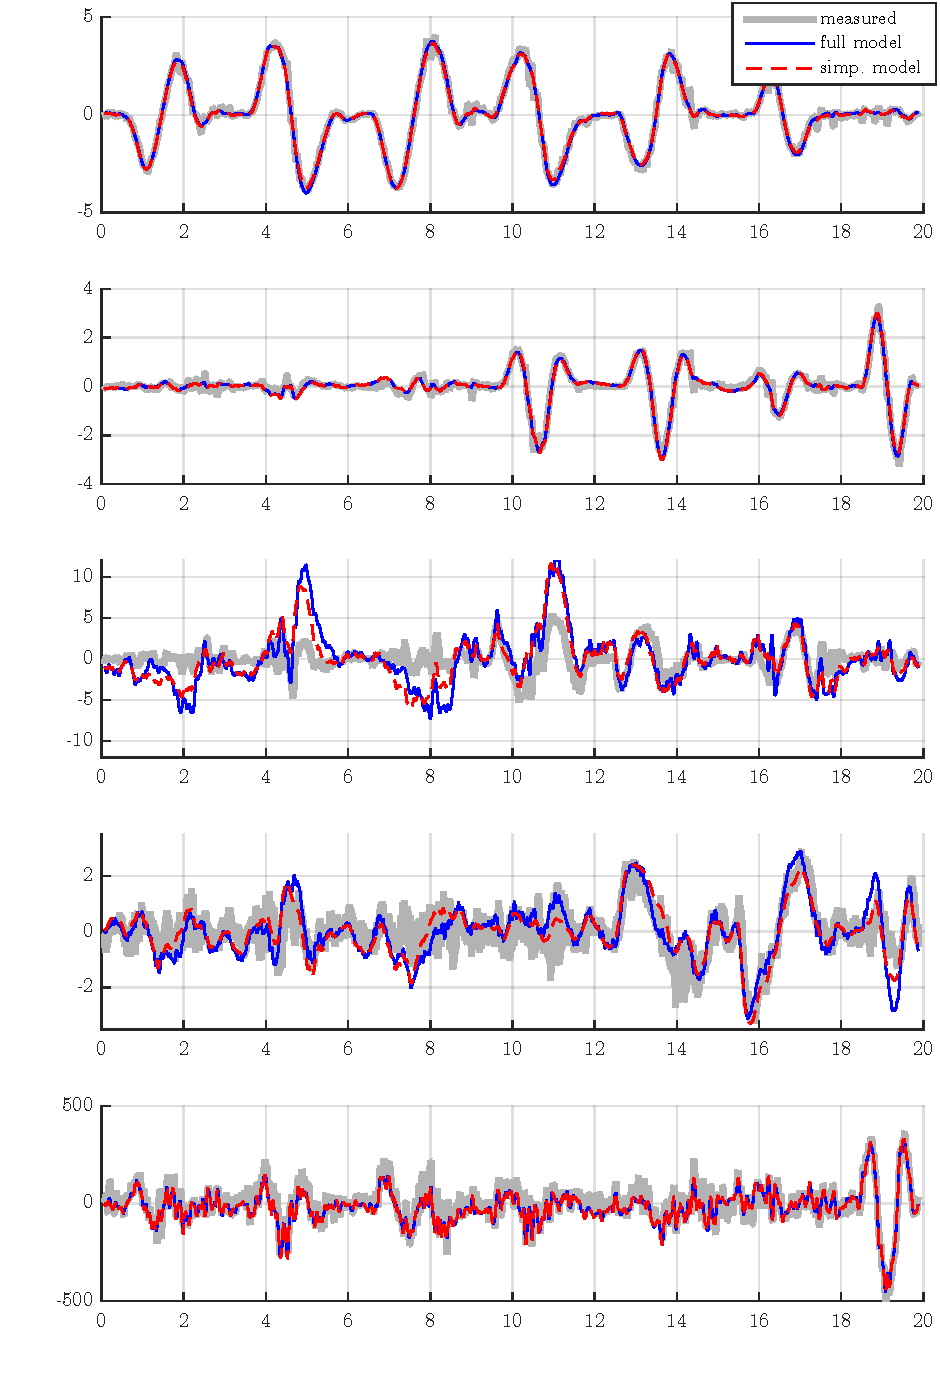
\includegraphics{ModelValidationTri.pdf}}%
\put(1.029882, 21.334540){\rotatebox{90}{\makebox(0,0)[t]{\smash{$\vxd$ in $\sfrac{\unit{m}}{\unit{s}^2}$}}}}%
\put(8.645781, 0.326348){\makebox(0,0)[b]{\smash{$t$ in $\unit{s}$}}}%
\put(0.677103, 2.890182){\rotatebox{90}{\makebox(0,0)[t]{\smash{$\PropVeld[1]$ in $\sfrac{\unit{RAD}}{\unit{s}^2}$}}}}%
\put(1.029882, 7.501271){\rotatebox{90}{\makebox(0,0)[t]{\smash{$\wzd$ in $\sfrac{\unit{RAD}}{\unit{s}^2}$}}}}%
\put(0.853493, 12.125590){\rotatebox{90}{\makebox(0,0)[t]{\smash{$\wyd$ in $\sfrac{\unit{RAD}}{\unit{s}^2}$}}}}%
\put(1.029882, 16.723451){\rotatebox{90}{\makebox(0,0)[t]{\smash{$\vzd$ in $\sfrac{\unit{m}}{\unit{s}^2}$}}}}%
\end{picture}%
\endgroup%%
 \caption{Model vs. measured accelerations for the Tricopter}
 \label{fig:ValidationTricopter}
\end{figure}

For the simplified model of the Tricopter we drop all off diagonal entries in the system inertia matrix $\sysInertiaMat$.
This means in particular $\bodyCOM{}{}{} = 0$ and $\bodyMOI{}{}{} = \diag(\Jx, \Jy, \Jz)$.
Furthermore we drop the damping parameters $\lz=0$, $\sigx=\sigz=0$ and assume isotropic translational damping $D_v = \DampingSym \idMat[3]$ with $\DampingSym = \tfrac{1}{3}(2\dvx + \dvz)$.
The resulting model equations are summarized as follows:

\begin{RedBox}
\textbf{Simplified Tricopter model.}
Rigid body dynamics
\begin{subequations}\label{eq:TricopterSimpModel}
\begin{align}
 \rd &= \R\, \v,&
 \m\vd + \wedOp(\w) m\v + \bodyDamping{}{} \v - \RT (\m\gravityAcc) &= \F + \FB,
% \FBd &= 0,
\\
 \Rd &= \R \wedOp(\w),&
 \J \dot{\w} + \wedOp(\w) \J \w &= \tau + \tauB,
% \tauBd &= 0
\end{align}
Generalized force from propellers
\begin{align}\label{eq:TriActuatorTrafo}
 \underbrace{\begin{bmatrix}[1.2] \Fx \\ \Fy \\ \Fz \\ \taux \\ \tauy \\ \tauz \end{bmatrix}}_{\genForce}
 =
 \underbrace{\begin{bmatrix}[1.1] 
  0 & 0 & 0 & \tfrac{\sqrt{3}}{2} & 0 & -\tfrac{\sqrt{3}}{2} \\
  0 & 0 & 0 & -\tfrac{1}{2} & 1 & -\tfrac{1}{2} \\
  1 & 1 & 1 & 0 & 0 & 0 \\
   \tfrac{\sqrt{3}\,\ArmRadius}{2} & 0 & -\tfrac{\sqrt{3}\,\ArmRadius}{2} & \tfrac{\ArmHeight}{2} + \tfrac{\sqrt{3}\,\kappaT}{2\,\kappaF} & \ArmHeight & \tfrac{\ArmHeight}{2} + \tfrac{\sqrt{3}\,\kappaT}{2\,\kappaF} \\
  -\tfrac{\ArmRadius}{2} & \ArmRadius & -\tfrac{\ArmRadius}{2} & \tfrac{\sqrt{3}\,\ArmHeight}{2} - \tfrac{\kappaT}{2\,\kappaF} & \tfrac{\kappaT}{\kappaF} & \tfrac{\kappaT}{2\,\kappaF} - \tfrac{\sqrt{3}\,\ArmHeight}{2} \\
  \tfrac{\kappaT}{\kappaF} & -\tfrac{\kappaT}{\kappaF} & -\tfrac{\kappaT}{\kappaF} & -\ArmRadius & -\ArmRadius & -\ArmRadius
 \end{bmatrix}}_{B}
 \underbrace{\begin{bmatrix}[1.2] \F^{\mathsf{V}}_1 \\ \F^{\mathsf{V}}_2 \\ \F^{\mathsf{V}}_3 \\ \F^{\mathsf{H}}_1 \\ \F^{\mathsf{H}}_2 \\ \F^{\mathsf{H}}_3 \end{bmatrix}}_{\F^\mathsf{VH}}
\\
 \F^{\mathsf{V}}_j = \PropForce[j] \cos\aServo[j], 
 \quad
 \F^{\mathsf{H}}_j = \PropForce[j] \sin\aServo[j],
 \quad
 \PropForce[j] = \kappaF \PropVel[j]^2, \qquad j=1,2,3
\end{align}
Propeller drive dynamics
\begin{align}
 \PropVeld[j] + \PropParam[1] \PropVel[j]^2 = \PropParam[2] \BLDCCurr[j] - \PropParam[3], \qquad j=1,2,3.
\end{align}
Servo dynamics
\begin{align}\label{eq:TriModelServoDynamics}
 \aServodd[j] + \ServoParam[1] \aServod[j] + \ServoParam[0] \aServo[j] = \ServoParam[0] \aServoU[j], \qquad j=1,2,3.
\end{align}

\end{subequations}
\end{RedBox}

Comparing the computed accelerations flight test in \autoref{fig:ValidationTricopter} leads to the following conclusions:% that the simplified model is as good or bad as the full model.
For the translational $\vxd$, $\vzd$ and the propeller acceleration $\PropVeld[1]$ the two models can not be distinguished and they match the measured accelerations quite well.
For the angular accelerations $\wxd$ and $\wzd$ the models differ slightly.
Unfortunately, one cannot say that the full model matches the measured accelerations better than the simplified.
This means that there are unmodeled effects that have a greater influence than the ones we dropped for the simplified model.
Overall the simplified model \eqref{eq:TricopterSimpModel} captures the Tricopter dynamics reasonably well and is due to its simplicity a good starting point for the model based control design.

\paragraph*{Quadcopter.}
Neglect the inertial couplings between the center body and propeller except $\PropInertia H_1 \PropVeld$.
Assume $\bodyCOM{}{}{} = 0$ and $\bodyMOI{}{}{} = \diag(\Jx, \Jx, \Jz)$.

\begin{RedBox}
Rigid body dynamics
\begin{subequations}
\begin{align}
 \rd &= \R\, \v,&
 \m \vd + \wedOp(\w) \m \v + \bodyDamping{}{} \v - \RT (\m\gravityAcc) &= \Fz e_3 + \FB,
% \FBd &= 0,
\\
 \Rd &= \R \wedOp(\w),&
 \J \dot{\w} + \wedOp(\w) \J \w &= \tau + \tauB,
% \tauBd &= 0
\end{align}
Generalized force from propeller rotation
\begin{align}\label{eq:QuadActuatorTrafo}
 \underbrace{\begin{bmatrix} \Fz \\ \taux \\ \tauy \\ \tauz \end{bmatrix}}_{\genForce}
 =
 \underbrace{\begin{bmatrix}
  1 & 1 & 1 & 1 \\
  0 & \ArmRadius & 0 & -\ArmRadius \\
  -\ArmRadius & 0 & \ArmRadius & 0 \\
  -\tfrac{\kappaT}{\kappaF} & \tfrac{\kappaT}{\kappaF} & -\tfrac{\kappaT}{\kappaF} & \tfrac{\kappaT}{\kappaF} \\
 \end{bmatrix}}_{B}
 \underbrace{\begin{bmatrix} \kappaF \PropVel[1]^2 \\ \kappaF \PropVel[2]^2 \\ \kappaF \PropVel[3]^2 \\ \kappaF \PropVel[4]^2 \end{bmatrix}}_{\PropForce[]}
 -
 \begin{bmatrix} 0 \\ 0 \\ 0 \\ \JP (\PropVeld[1] - \PropVeld[2] + \PropVeld[3] - \PropVeld[4]) \end{bmatrix}
\end{align}
Propeller drive dynamics
\begin{align}\label{eq:QuadPropDynamics}
 \PropInertia \PropVeld[j] + \kappaT \PropVel[j]^2 = \BLDCTorqueConstant[j] \BLDCCurr[j] - \BLDCFriction[j], \qquad j=1,\ldots,4.
\end{align}
\end{subequations}
\end{RedBox}


\begin{figure}
 \centering
 \footnotesize%
 \appendtographicspath{{graphics/ModelValidationQuad/}}%
 \begingroup%
\setlength{\unitlength}{1cm}%
\begin{picture}(15.900000,23.300000)%
\put(0,0){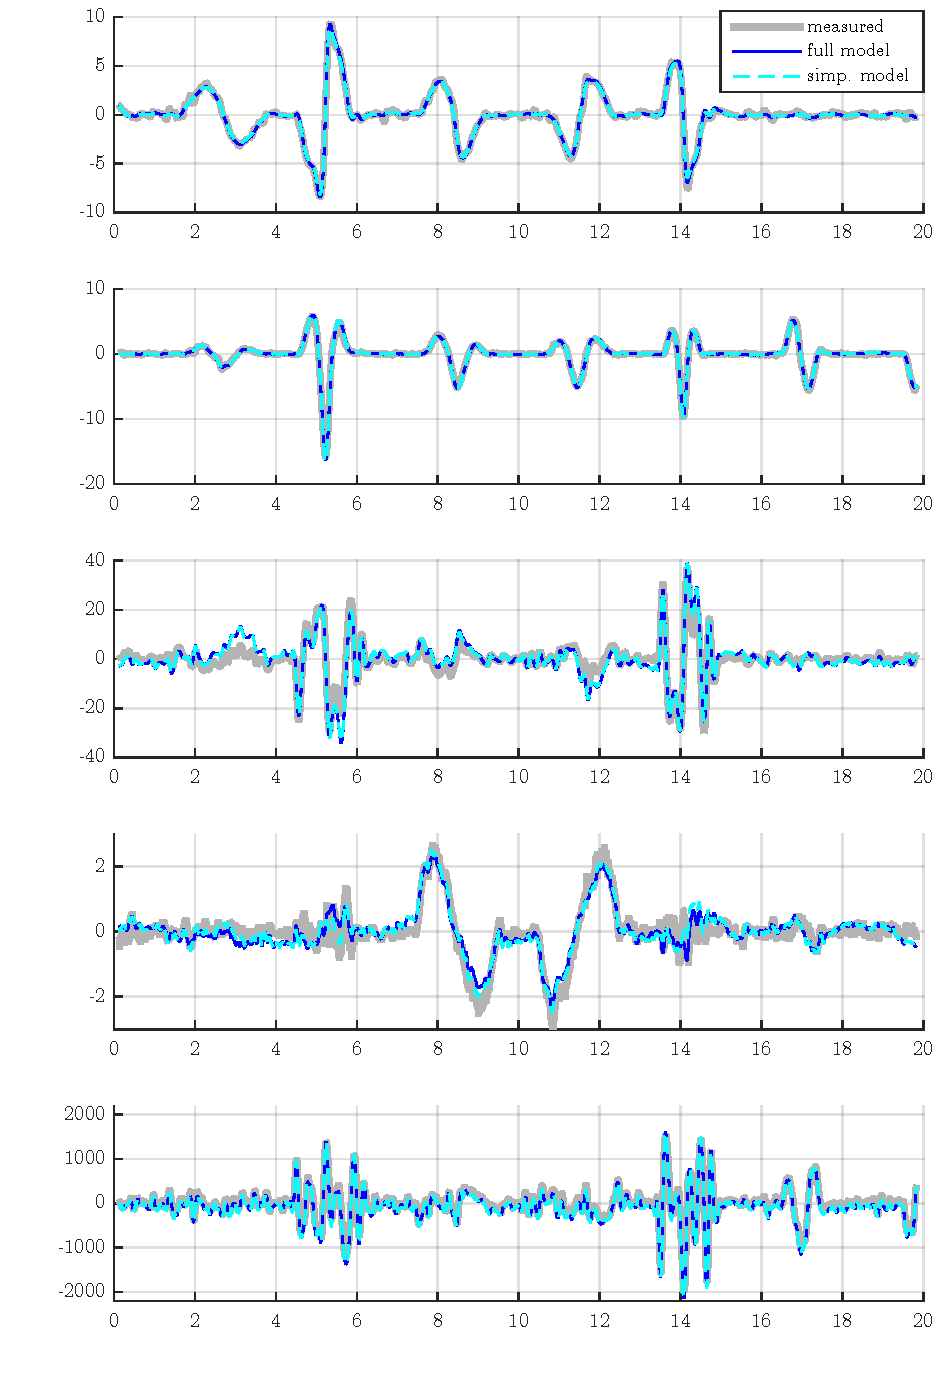
\includegraphics{ModelValidationQuad.pdf}}%
\put(0.710903, 7.501271){\rotatebox{90}{\makebox(0,0)[t]{\smash{$\wzd$ in $\sfrac{\unit{RAD}}{\unit{s}^2}$}}}}%
\put(8.750137, 0.326348){\makebox(0,0)[b]{\smash{$t$ in $\unit{s}$}}}%
\put(0.710903, 2.890182){\rotatebox{90}{\makebox(0,0)[t]{\smash{$\PropVeld[1]$ in $\sfrac{\unit{RAD}}{\unit{s}^2}$}}}}%
\put(0.710903, 12.125590){\rotatebox{90}{\makebox(0,0)[t]{\smash{$\wyd$ in $\sfrac{\unit{RAD}}{\unit{s}^2}$}}}}%
\put(0.710903, 16.723451){\rotatebox{90}{\makebox(0,0)[t]{\smash{$\vzd$ in $\sfrac{\unit{m}}{\unit{s}^2}$}}}}%
\put(0.710903, 21.334540){\rotatebox{90}{\makebox(0,0)[t]{\smash{$\vxd$ in $\sfrac{\unit{m}}{\unit{s}^2}$}}}}%
\end{picture}%
\endgroup%%
 \caption{Model vs. measured accelerations on the quadcopter}
\end{figure}